\section{The Pyramid Model}

\begin{figure}[h]
\centering
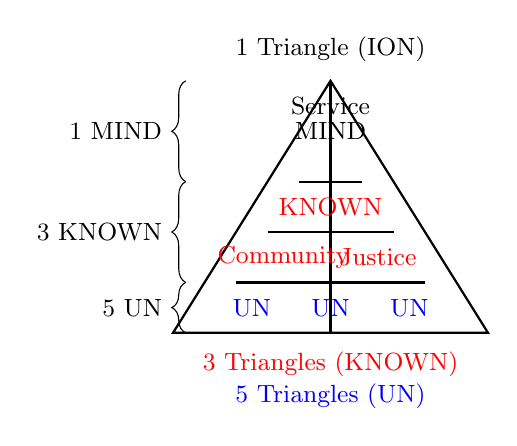
\begin{tikzpicture}[scale=0.8, every node/.style={align=center, font=\small}]

% Main pyramid outline (2D view)
\draw[thick] (0,0) -- (5,0) -- (2.5,4) -- cycle;

% Horizontal divisions
\draw[thick] (1,0.8) -- (4,0.8); % Level 1
\draw[thick] (1.5,1.6) -- (3.5,1.6); % Level 2
\draw[thick] (2,2.4) -- (3,2.4); % Level 3

% Vertical divisions to create triangles
\draw[thick] (2.5,4) -- (2.5,0); % Center line

% Label the sections
% Top section (MIND - 1 triangle)
\node at (2.5,3.2) {MIND};
\node at (2.5,3.6) {Service};

% Middle section (KNOWN - 3 triangles)
\node[red] at (2.5,2.0) {KNOWN};
\node[red] at (1.75,1.2) {Community};
\node[red] at (3.25,1.2) {Justice};

% Bottom section (UN - 5 triangles)  
\node[blue] at (2.5,0.4) {UN};
\node[blue] at (1.25,0.4) {UN};
\node[blue] at (3.75,0.4) {UN};

% Add labels for the triangle counts
\node at (2.5,4.5) {1 Triangle (ION)};
\node[red] at (2.5,-0.5) {3 Triangles (KNOWN)};
\node[blue] at (2.5,-1.0) {5 Triangles (UN)};

% Add braces to show the sections
\draw[decorate,decoration={brace,amplitude=5pt},yshift=0pt] 
(0.2,0) -- (0.2,0.8) node[midway,left=5pt] {5 UN};
\draw[decorate,decoration={brace,amplitude=5pt},yshift=0pt] 
(0.2,0.8) -- (0.2,2.4) node[midway,left=5pt] {3 KNOWN};
\draw[decorate,decoration={brace,amplitude=5pt},yshift=0pt] 
(0.2,2.4) -- (0.2,4) node[midway,left=5pt] {1 MIND};

\end{tikzpicture}
\caption{The Pyramid Model: 5 UN + 3 KNOWN + 1 MIND = Complete Structure}
\label{fig:pyramid}
\end{figure}

In the pyramid model, the five triangles at the bottom (UN) represent the foundation, the three middle triangles (KNOWN) represent community, service, and justice, and the single top triangle represents the MIND. Your Mind is the strongest at the top and it knows the three triangles in the middle. You must trust the middle triangles to truly understand the UN. When the mind's eye understands the five unknown triangles, this is called EPIPHANY or feeling.